% Instructions to change to html version:
% Comment out:
%  minipage, multicols,columnbreak, mathbf, hrule
% Replace all: \begin{minipage}% %%%%\end{minipage} %%%%%%%\begin{mulicols}  %%%%%%\end{mulicols}  %%%%%\columnbreak % %%%%%\begin{framed} %%%%%%\end{framed} %%%\hrule
% Search for  
% Replace \\] with \[ and \) with \(
% Enclose graphics in figure environments and add captions
% Re-tag \df environments as sections, subsections, etc.
% Command Line Code to Create html version:
%First: pdflatex -shell-escape filename.tex                                   
%Second, for each figure: inkscape "filename-figure1.pdf" -o "filename-figure1.png"
% Third: htlatex filename.tex "ht5mjlatex.cfg, charset=utf-8" " -cunihtf -utf8"


\documentclass[10pt]{article}

%\usepackage{tikz, pgf,pgfplots,wasysym,array}
%\usepackage{wasysym}

\usepackage{amsmath,amssymb}

\ifdefined\HCode
  \def\pgfsysdriver{pgfsys-tex4ht-updated.def}
\fi 
%\ifdefined\HCode
%  \def\pgfsysdriver{pgfsys-dvisvgm4ht.def}
%\fi 
\usepackage{tikz}
\usetikzlibrary{calc,decorations.markings,arrows}
\usepackage{pgfplots}

\pgfplotsset{compat=1.12}
\usepackage{myexternalize}
%\usetikzlibrary{calc,decorations.markings,arrows}
\usepackage{framed}
\usepackage[none]{hyphenat}

\input{../../../common/1336_header_test.tex}

\begin{document}

\everymath{\displaystyle}

\renewcommand{\myTitle}{MATH 2330: Multivariable Calculus}

\renewcommand{\mySubTitle}{Section 5.5: Cylindrical \& Spherical Coordinates}
%~\hfill Name: \underline{~~~~~~~~~~~~~~~~~~~~~~~~~~~~~~~~~~~~~~~~~~~~~~~}

\lectTitle{\vspace*{-.5in}\myTitle}{\vspace*{.1in}\mySubTitle \vspace*{-.25in}}



\section*{Cylindrical Coordinates}

%\setlength{\columnseprule}{0.4pt}
%\setlength{\columnsep}{3em}

%\hspace*{-.8in}%\begin{minipage}{1.25\textwidth}
%\begin{framed}

%\begin{multicols}{2}

%\df{\textcolor{sblack}{Cylindrical Coordinates:}}

%\begin{minipage}{.3\textwidth}
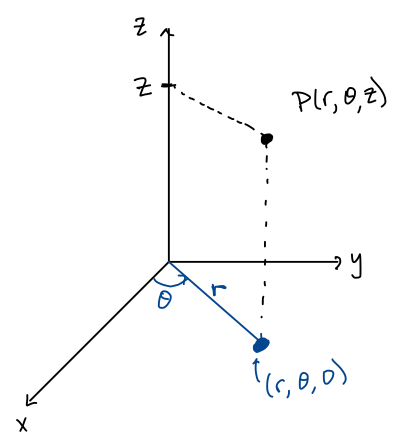
\includegraphics[width=\textwidth]{Ch12s6-Cylindrical-Coordinates.png}
%\end{minipage}
\hspace*{.4in}
%\begin{minipage}{.6\textwidth}
\subsection*{Equations:}

\[x=r\cos\theta, \qquad y=r\sin\theta, \qquad z = z, \qquad x^2+y^2=r^2\]


\vspace*{.2in}

\subsubsection*{Triple Integral Setup:}
\textbf{Integrate with respect to \(z\) first, and be sure to replace all \(x\)'s and \(y\)'s.}
\[
\iiint_{E} f(x,y,z)\ dV = \iint_{D} \left(\int_{u_1(x,y)}^{u_2(x,y)} f(x,y,z)\ dz\right) dA
\]

\[
\qquad \qquad =\int_\alpha^\beta \int_{h_1(\theta)}^{h_2(\theta)} \int_{u_1(r\cos\theta, r\sin\theta)}^{u_2(r\cos\theta, r\sin\theta)} f\left(r\cos\theta, r\sin\theta,z\right) r dzdrd\theta
\]

\textbf{Volume Element: }\({dV = r\ dz\ dr\ d\theta}\)
%\end{minipage}

%%\columnbreak


%\end{multicols}

%\end{framed}

%\end{minipage}



%\section*{Examples:}


\begin{enumerate}[{Example} 1: ]
%\item Revisit ``Fun with Polar Volume'' Problem 2.


\item Revisit finding the volume of the ``Ice Cream Cone'' solid region bounded above by \(x^2+y^2+z^2=4\) and below by \(x^2+y^2 = z^2\), where \(z\geq 0\).


\end{enumerate}

\pagebreak

\section*{Spherical Coordinates}

%\setlength{\columnseprule}{0.4pt}
%\setlength{\columnsep}{3em}

\hspace*{-.8in}%\begin{minipage}{1.25\textwidth}
%\begin{framed}

%\begin{multicols}{2}

%\df{\textcolor{sblack}{Spherical Coordinates:}}

%\begin{minipage}{.3\textwidth}
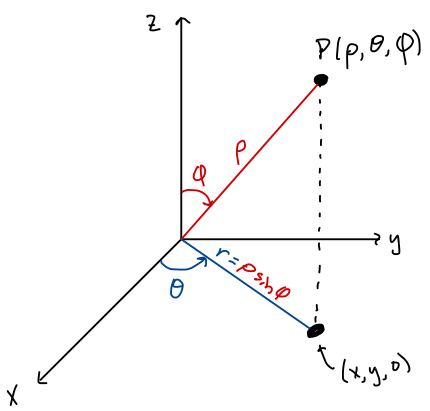
\includegraphics[width=\textwidth]{Ch12s7-Spherical-Coordinates.png}
%\end{minipage}
\hspace*{.4in}
%\begin{minipage}{.6\textwidth}
\subsection*{Variables:}
\begin{itemize}
\item \(\rho\): distance from the origin \(\rho^2 = x^2+y^2+z^2\), \(\rho \geq 0\)
\item \(\theta\): same angle as in polar/cylindrical coordinates, \(0\leq \theta\leq 2\pi\)
\item \(\phi\): angle measured down from the positive \(z-\)axis, \(0\leq \phi\leq \pi\)
\end{itemize}
~\\

\subsubsection*{Equations:}

\[x=\rho\sin\phi \cos\theta, \qquad y=\rho\sin\phi\sin\theta, \qquad z = \rho\cos\phi, \qquad x^2+y^2+z^2=\rho^2\]


%\end{minipage}

\vspace*{.1in}
\hrule
\vspace*{.2in}


\subsubsection*{Triple Integral Setup:}
For a solid region \({E}\) with bounds:
\(\qquad \rho:\ a\ \text{to}\ b, \qquad \theta:\ \alpha\ \text{to}\ \beta, \qquad \phi:\ c\ \text{to}\ d\)

\[
\iiint_{E} f(x,y,z)\ dV 
=\int_c^d\int_\alpha^\beta \int_a^b  f\left(\rho\sin\phi\cos\theta, 
\rho\sin\phi\sin\theta,\rho\cos\phi\right) \rho^2\sin\phi\ d\rho\ d\theta\ d\phi
\]

\textbf{Volume Element: }\({dV = \rho^2\sin\phi\ d\rho\ d\theta\ d\phi}\)

%\vspace*{.1in}
%\hrule
%\vspace*{.2in}

%\end{framed}

%\end{minipage}


\begin{enumerate}[{Example} 1: ]
%\item Revisit ``Fun with Polar Volume'' Problem 2.

\item How would you describe a sphere of radius \(R\) using spherical coordinates? Top only? Bottom only? First octant only?

\vfill

\item Find the volume of the region described by \(1\leq x^2+y^2+z^2\leq 9\) using a triple integral.
\vfill

\item Revisit finding the volume of the ``Ice Cream Cone'' solid region bounded above by \(x^2+y^2+z^2=4\) and below by \(x^2+y^2 = z^2\), where \(z\geq 0\).

\vfill

\item %Integrate \(f(x,y,z)=z\) over the ``Ice Cream Cone'' solid region described above.\\
What does the following quantity represent? Calculate it for the ``Ice Cream Cone'' solid region described above.
\[\frac{\displaystyle \iiint_{E} z\ dV}{\displaystyle \iiint_{E}  dV}\]


\end{enumerate}

\pagebreak
\section*{Equations of Some ``Standard'' Surfaces:}

%\begin{framed}


\subsection*{Cylinder of radius a:}
%\begin{multicols}{2}
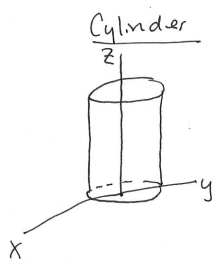
\includegraphics[height=2in]{Ch12s7-Cylinder.png}

%\columnbreak

\begin{itemize}
\item \textbf{Rectangular Coordinates:} \(x^2+y^2=a^2\)
\item \textbf{Cylindrical Coordinates:} \(r=a\)
\item \textbf{Spherical Coordidnates:} (Not worth it!)
\end{itemize}
%\end{multicols}

%\vspace*{.1in}
%\hrule
%\vspace*{.2in}

\subsection*{Cone (top half):}
%\begin{multicols}{2}
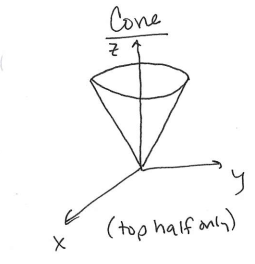
\includegraphics[height=2in]{Ch12s7-Cone.png}

%\columnbreak

\begin{itemize}
\item \textbf{Rectangular Coordinates:} \(z=\sqrt{x^2+y^2}\)
\item \textbf{Cylindrical Coordinates:} \(r=z\)
\item \textbf{Spherical Coordidnates:} \(\phi = \frac{\pi}{4}\)
\end{itemize}
%\end{multicols}
%
%%\vspace*{.1in}
%\hrule
%\vspace*{.2in}

\subsection*{Sphere of radius a:}
%\begin{multicols}{2}
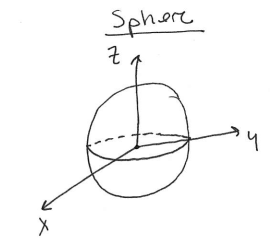
\includegraphics[height=2in]{Ch12s7-Sphere.png}

%\columnbreak

\begin{itemize}
\item \textbf{Rectangular Coordinates:} \(x^2+y^2+z^2=a^2\)
\item \textbf{Cylindrical Coordinates:} \(r^2+z^2 = a^2\)
\item \textbf{Spherical Coordidnates:} \(\rho=a\)
\end{itemize}
%\end{multicols}

%\end{framed}

%%\end{minipage}

\end{document}

